% File name: report/repord.tex

\documentclass[a4paper,11pt]{article}  % Standard document class
\usepackage[english]{babel}            % Set document language
\usepackage{fullpage}                  % Set up page for small margins etc

\usepackage{graphicx}                  % For including images in document
%\usepackage{placeins}                  % Allows use of \FloatBarrier
% to avoid images or tables
% moving into next section
%\usepackage{subfig}                    % For subfigures...

\usepackage{amsmath}                   % For improving maths/formula typesetting
%\usepackage{tabularx}                  % Table changing package

%\usepackage{algpseudocode}             % For producing algorithms/flowcharts

\usepackage{listings}                  % For including source code in document
\lstset{
  basicstyle = \small
}

% Provide command for scientific notation
\providecommand{\e}[1]{\ensuremath{\times10^{#1}}}
\providecommand{\degrees}{\ensuremath{^{\circ}}}

% Define title here:
\title{4th Year Project: Soldering Machine}
\author{James Glanville}
\date{11th June 2013}

\begin{document}

% generate title
\maketitle

\section{Existing Solutions}
There are a number of hobbyist solutions to deal with SMD parts:

\begin{itemize}
	\item	Solder paste + heat:
		\begin{itemize}
			\item	Solder stencils: Expensive setup costs, very quick to use. Not suitable for
				this project.
			\item	Manual solder paste application: Mostly expensive dispenser, or with a syringe.
			\item	Hot air gun: Can be relatively difficult to get the right temperature profile.
			\item	Converted toaster over: seems quite common.
		\end{itemize}

	\item	Soldering by hand:
		\begin{itemize}
			\item	Dragging a bead of solder along pins, then cleaning up with solder sucker/wick.
				This requires a lot of feedback, which is difficult to automate.
			\item	Some devices (SOIC?) have slightly bendy pins. A small amount of downwards 
				pressure on the pin onto a tinned pad works.
		\end{itemize}
\end{itemize}

\section{Project Idea}
When finished, the machine should be able to be connected to a computer via a USB port. A custom GUI will load the necessary 
design files (for example the holes to be drilled, pads to be soldered), generate the necessary GCODE, and send it to the printer.

\section{Requirements}

\subsection{X/Y axes}
A device pitch of 0.4mm (distance from centre of one pin to the next) is on the lower end of SMD ICs. Using solder paste,
devices will shift slightly upon heating to self-align. A requirement is that the device should be placed to a
small fraction of its pitch, so there is no danger of incorrect connections. I have decided to aim for an accuracy of +-0.05mm
in placement. This should be sufficient, but may be difficult to achieve in practice.

\subsection{Board size}
A maximum board size of 100x100mm would be sufficient for the vast majority of boards. I have chosen 100x100mm because that
is the maximum board size using the free version of EAGLE, a popular design package. As a result, there are a lot of designs
that use the maximum size, and it would be useful if this project allowed those designs to be populated.

\section{Design}

\subsection{X/Y axes}

The X/Y axes have the same requirements: +-0.05mm accuracy. There is the choice between moving the various tools over a stationary
bed, or keeping the tools stationary and moving the bed. I have decided to move only the bed, because it means that the pick
and place functionality does not have to move the parts, simply lift and lower them. This should reduce the risk of the parts
shifting on the needle, or falling off. It also allows for the use of more tools since weight is no longer a concern.

Driving mechanisms:

\begin{itemize}
	\item	Toothed belts + pulleys + stepper motors: Simple, as used in reprap 3d printers. Can be run open loop
		very easily. Requires: stepper motor + driver, belt, pulley.
	\item	Threaded rod + stepper motors: Cheap, slower but probably fast enough. M3-5 easy to couple
		to motor shafts (http://www.thingiverse.com/thing:9622).
	\item	Closed loop: dc motors + feedback. Linear potentiometers: relatively expensive, and potential
		issues with electrical noise. Rotary encoders: cheap, accurate (m4 pitch is ~0.5mm, not much
		travel/turn, might only need 10 slot encoder)

\end{itemize}

Linear slides:

\begin{itemize}
	\item	Drawer slides: cheap, surprisingly high precision.
	\item	3d printed bushings + steel rod. If 3d printer existance assumed, then very cheap solution.
	\item	LM8UUs (or smaller): About £1 each, so probably too expensive.
\end{itemize}

\subsection{Z axis}
The Z axis will not require as much precision as the X and Y. Potential mechanisms:

\begin{itemize}
	\item	Micro servos: cheap (£2 on ebay). Require no drivers, and simple to drive. Z axis potentially
		does not need to be linear (UP/DOWN only?) so rotary-\textgreater linear mechanism simpler. If not linear,
		then hinging out of the way is a cheaper mechanism than slides.
\end{itemize}

\subsection{Part placement}

\begin{itemize}
	\item	Manual placement. Much more of a problem for a large number of SMD resistors/capacitors etc, than
		larger components. 
	\item	Vacuum "tweezers". Mechanically relatively simple, but problems of intelligent control, as well
		as well as storing the components before placement. As an experiment, I tried using an aquarium pump
		in reverse (by attaching the silicone tubing to the inlet instead of the outlet) connected to a fairly
		large diameter needle (ID: Xmm).
\end{itemize}

\subsection{Heated Bed}
Soldering to a hot board is easier (smaller temperature difference). Probably not worth the cost/complexity.

\subsection{Flux application}
Flux application may be a significant problem, unless a manual brush with a solder pen is sufficient.

\subsection{Drilling and isolation routing}
Isolation routing is a method to mill traces from copper-clad pcb. A conical engraving bit is used to cut very narrow tracks through
the copper, to leave disconnected pads as required. 

Drilling holes in pcbs is a time-consuming process to do by hand. If this machine could drill the holes automatically,
it would reduce the total time taken significantly. A small brushless motor with a collet would be enough. The biggest challenge
will be mechanically coupling the motor to the drill bit. This is not intrinsically difficult, but it should be made in a way that
is accessable to people without the use of a lathe (?)

A 25 Amp ESC (Turnigy plush 25A, £9) powering a small brushless motor (Turnigy 2217 20turn 860kv 22A outrunner, £10) is capable of milling
steel easily, so smaller, cheaper motors should be fine for routing/drilling copper.

An alternative design would be to use a low cost rotary tool, which already has the bearings, collet and spindle motor. 

\subsection{Soldering iron}
Designing a mount for a cheap and widely available soldering iron may well be cheapest. 

\subsection{Electronics/Firmware}
I have decided to use an avr chip to translate GCODE to stepper motor commands for the following reasons:
\begin{itemize} \itemsep0em
	\item	Cost: an atmega328 is £2-3, a usb-serial chip is <£2, which is not much.
	\item	Mature open source firmware (GRBL, https://github.com/grbl/grbl) is available for gcode-\textgreater stepper
		conversion, which leaves more time to focus on other parts of this project.
\end{itemize}


\section{Tools}
I have a small mill, a 3d printer and a lathe. It may be worth considering that a lot of people/schools have
access to a laser cutter and perhaps mill/lathe, so if possible all custom components could be 3d printed or 
lasercut.

\section{Vacuum Placing}
\subsection{Prototype}
To test how effectively small parts could be placed with a vacuum, I made a simple test setup:

\begin{itemize} \itemsep0em
	\item	12V diaphragm air pump (£8.89 - ebay)
	\item	6mm OD/4mm ID silicone tube (£2.69/m - ebay)
	\item	various needles (need more info here)
	\item	MOSFET
	\item	330$\Omega$ resistor
\end{itemize}

\begin{figure}[ht!]
\centering
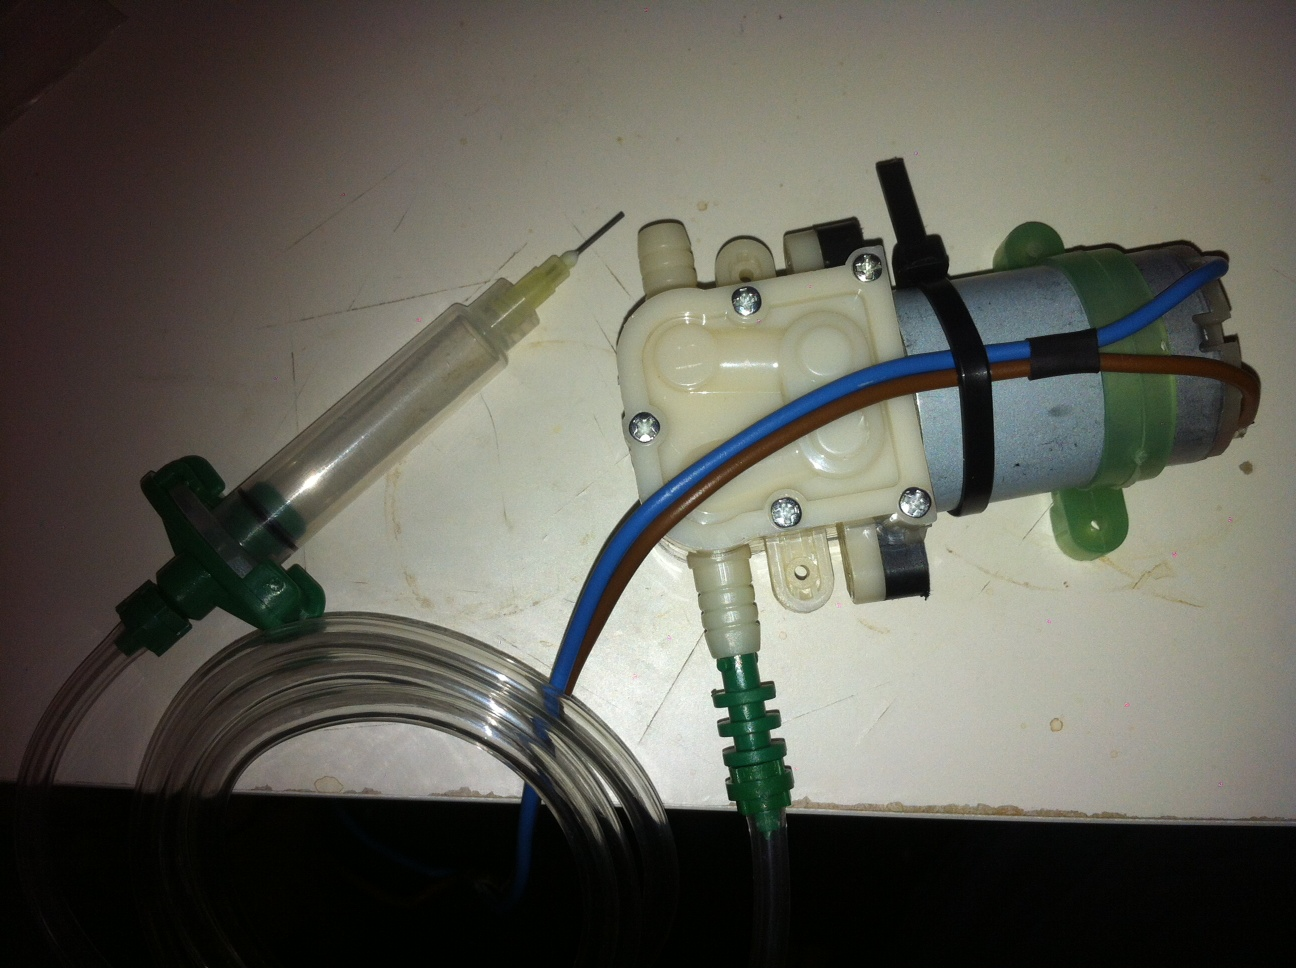
\includegraphics[width=90mm]{resources/pump_and_hose.jpg}
\caption{Pump with hose and needle.}
\label{hose and needle}
\end{figure}

The pump draws ~200mA at 12V, which is easily controlled with a MOSFET. Using a 1.8mm ID needle, SOIC-20 parts were picked up, and had significant friction against the needle - essential to avoid slipping or rotating. It was important to place the needle as centrally as possible on the part to avoid generating any imbalance that allowed the part to fall. 

\subsection{Conclusions}
A vacuum needle solution is workable, and a good choice for this project. Things that need to be considered for use in the final project:

\begin{itemize}
	\item	The pump takes a certain time to generate a vacuum because of the relatively large internal volume of the pump
		and silicon tube. It will be important to measure this, and add a margin of error so that full suction is applied
		to each device before any movement takes place. Similarly, when turning off the pump, the pressure must return to
		atmospheric before the device can be considered to have been placed succesfully. In testing, the pump I used took
		less than a second to leak sufficiently for this to occur, but if another pump were to be used, it may be necessary
		to place a tiny hole in the air line so that pressure drops quickly.
	\item	It is important to place the needle very near to the centre of mass of the device. The majority of devices will be
		symmetrical, which will make this easier.
	\item	The needle must be able to be raised and lowered to the correct heights. It may be possible to push the needle down
		with a weak spring, with a micro servo that raises it - this would remove any need to know the exact height of each
		device. This will need to be tested.
\end{itemize}

\begin{figure}[ht!]
\centering
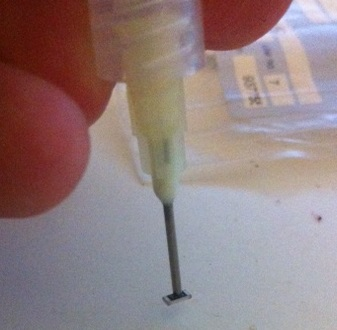
\includegraphics[width=90mm]{resources/needle_with_resistor.jpg}
\caption{SMD resistor being picked up.}
\label{overflow}
\end{figure}
\end{document}
